\documentclass[11pt,twocolumn]{article}

\usepackage{array}
\usepackage[url=false, doi=false]{biblatex}
\usepackage{booktabs}
\usepackage[font=footnotesize, labelfont=bf]{caption}
\usepackage{enumitem}
\usepackage[symbol]{footmisc}
\usepackage[scale=0.85]{geometry}
\usepackage{graphicx}
\usepackage{microtype}
\usepackage{multirow}
\usepackage{parskip}
\usepackage{siunitx}
\usepackage{subcaption}
\usepackage{titlesec}
\usepackage[dvipsnames]{xcolor}
\usepackage{xurl}
\usepackage{amsmath}

\usepackage[hidelinks]{hyperref}
\usepackage[nameinlink,capitalise]{cleveref}

\addbibresource{../bibliography.bib}

\titlelabel{}

\newcommand{\atom}[1]{\colorbox{Gray!30}{\ttfamily #1}}
\newcommand{\citen}[1]{~\parencite{#1}}
\newcommand{\citeay}[1]{\textcite{#1}}

\title{A Strategy Zoo for Dynamic LeanCoP Control}
\date{}
\author{}

\begin{document}
\twocolumn[
	\centering
	\vspace{1em}
	{\LARGE Modifying LeanCoP Options on the Fly \par} \vspace{3pt}
	{\large (aka ``the PAAR/AITP paper'') \par}
	\vspace{2em}
]

\section{Introduction}

In LeanCoP, small changes to proof-search control have large practical effects\citen{ottenLeanCoP20,Otten2023leanCoP20}.
These variants are studied in a PyCoP-style environment with explicit proof actions, including \atom{cut}, \atom{comp(J)}, and \atom{Reset(n)}.

Fixed strategy schedules are already central to leanCoP-style prover engineering\citen{ottenLeanCoP20}, and recent work has treated schedule design itself as a learning problem\citen{mangla2022a,Mangla2025MLTPS}. The present experiments stay at the hand-designed level, but use that scheduling perspective throughout.

\section{Strategies}

The following strategies are used in the schedules.

\begin{description}[style=nextline, itemsep=-3pt, leftmargin=18pt]
	\item[FirstAction] The first legal action is selected\citen{letzModelEliminationConnection2001,ottenLeanCoP20}.
	\item[LeanCopCut] LeanCoP-style inclusive restricted backtracking is used: successful reductions and extensions are cut, and \atom{comp(7)} is used for completeness\citen{ottenLeanCoP20}.
	\item[ReductionCut] Inclusive cut is applied only on reductions\citen{farberCuriouslyEffectiveBacktracking2024}.
	\item[HeuristicReductionCut] Forward actions are ordered heuristically, preferring reductions and then shorter clauses; cut is applied only on reductions\citen{letzModelEliminationConnection2001,farberCuriouslyEffectiveBacktracking2024}.
	\item[SubgoalReordering] A stricter categorical order is used: reductions, then shorter extensions, then shorter starts\citen{letzModelEliminationConnection2001}.
	\item[EntropyCut] The baseline order is used, but \atom{cut} is added only when the softmax entropy of heuristic action scores is low\citen{zomboriRoleEntropyGuiding2021}.
	\item[AdaptiveReset] Dead-end backtracks are replaced by explicit resets to a larger depth bound, using a simple search-state heuristic\citen{HoldenSATQSAT,liReinforcementLearningBased2024}.
	\item[SmartCut] Entropy-based cut is combined with adaptive reset\citen{zomboriRoleEntropyGuiding2021,HoldenSATQSAT,liReinforcementLearningBased2024}.
\item[FewAlternativesCut] The default depth-first order and \atom{comp(7)} are used, but \atom{cut} is applied only when the current choice point is narrow\citen{ottenLeanCoP20,farberCuriouslyEffectiveBacktracking2024}.
\item[GoalDistanceCut] LeanCoP-style cut is used, but forward actions are ordered by an estimate of proximity to closure\citen{letzModelEliminationConnection2001}.
\item[DepthPhasedCut] Reductions are always cut, while extensions are cut only near the top of the iterative-deepening tree; \atom{comp(10)} is used\citen{ottenLeanCoP20}.
\end{description}

\newcommand{\NA}{{---}}

\begin{table*}
\centering
\footnotesize
\begin{tabular*}{\textwidth}{@{\extracolsep{\fill}}l S[table-format=4.0] S[table-format=3.0] S[table-format=3.0] S[table-format=3.0]}
\toprule
\multicolumn{1}{l}{Setting} &
\multicolumn{1}{r}{Solved} &
\multicolumn{1}{r}{Unsolved by \texttt{LeanCopCut}} &
\multicolumn{1}{r}{Unsolved by \texttt{FirstAction}} &
\multicolumn{1}{r}{Unsolved by both} \\
\midrule
\texttt{FirstAction} (60s) & 2049 & 174 & \NA & \NA  \\
\texttt{LeanCopCut} (60s) & 2164 & \NA & 289 & \NA  \\
\texttt{P1 60s} & 2291 & 171 & 323 & 64 \\
\texttt{P2 60s} & 2140 & 247 & 174 & 101 \\
\addlinespace
\texttt{FirstAction} (120s) & 2134 & 166 & \NA & \NA \\
\texttt{LeanCopCut} (120s) & 2304 & \NA & 336 & \NA \\
\texttt{P1 120s} & 2449 & 173 & 387 & 74 \\
\texttt{P2 120s} & 2292 & 256 & 227 & 113 \\
\bottomrule
\end{tabular*}
\caption{Solved-problem counts for the controls and the four portfolios.}
\label{tab:schedule-results}
\end{table*}

\section{Schedules}

\begin{description}[style=nextline, itemsep=5pt, leftmargin=18pt]
	\item[P1 60s] Maximises total solved problems.\par
	{\small\begin{tabular}{@{}r@{\ }l@{\hspace{0.75em}}r@{\,ms}}
	(1) & \texttt{AdaptiveReset} & \num{435} \\
	(2) & \texttt{SubgoalReordering} & \num{1917} \\
	(3) & \texttt{LeanCopCut} & \num{44495} \\
	(4) & \texttt{SmartCut} & \num{1228} \\
	(5) & \texttt{FirstAction} & \num{10295} \\
	(6) & \texttt{GoalDistanceCut} & \num{1626} \\
	\end{tabular}}
	\item[P2 60s] Maximises solved problems not solved by LeanCoP.
	\par
	{\small\begin{tabular}{@{}r@{\ }l@{\hspace{0.75em}}r@{\,ms}}
	(1) & \texttt{SmartCut} & \num{863} \\
	(2) & \texttt{EntropyCut} & \num{37776} \\
	(3) & \texttt{GoalDistanceCut} & \num{9123} \\
	(4) & \texttt{HeuristicReductionCut} & \num{581} \\
	(5) & \texttt{AdaptiveReset} & \num{4588} \\
	(6) & \texttt{ReductionCut} & \num{2793} \\
	(7) & \texttt{SubgoalReordering} & \num{1917} \\
	(8) & \texttt{FewAlternativesCut} & \num{1749} \\
	\end{tabular}}
	\item[P1 120s] Maximises total solved problems.
	\par
	{\small\begin{tabular}{@{}r@{\ }l@{\hspace{0.75em}}r@{\,ms}}
	(1) & \texttt{SubgoalReordering} & \num{3705} \\
	(2) & \texttt{AdaptiveReset} & \num{4588} \\
	(3) & \texttt{LeanCopCut} & \num{95539} \\
	(4) & \texttt{HeuristicReductionCut} & \num{581} \\
	(5) & \texttt{EntropyCut} & \num{13619} \\
	(6) & \texttt{GoalDistanceCut} & \num{1584} \\
	(7) & \texttt{DepthPhasedCut} & \num{339} \\
	\end{tabular}}
	\item[P2 120s] Maximises solved problems not solved by LeanCoP.
	\par
	{\small\begin{tabular}{@{}r@{\ }l@{\hspace{0.75em}}r@{\,ms}}
	(1) & \texttt{SmartCut} & \num{863} \\
	(2) & \texttt{SubgoalReordering} & \num{13410} \\
	(3) & \texttt{DepthPhasedCut} & \num{31596} \\
	(4) & \texttt{HeuristicReductionCut} & \num{581} \\
	(5) & \texttt{GoalDistanceCut} & \num{1584} \\
	(6) & \texttt{EntropyCut} & \num{43111} \\
	(7) & \texttt{AdaptiveReset} & \num{4588} \\
	(8) & \texttt{ReductionCut} & \num{23446} \\
	\end{tabular}}
\end{description}

Time allocations are chosen by exact maximum-coverage optimisation, and slot order is chosen by exact optimisation of serial runtime.

\section{Results}


The violin plots in \cref{fig:violins} use the same score as in Mangla et al.\citen{Mangla2025MLTPS}.
With total budget $T$ and consumed time $t$, the score is
\[
s =
\begin{cases}
	0.5 + \frac{T - t}{2T} & \text{on success,} \\[3pt]
	\frac{T - t}{2T} & \text{otherwise.}
\end{cases}
\]

\begin{figure*}[t]
\centering
\begin{subfigure}{\linewidth}
\centering
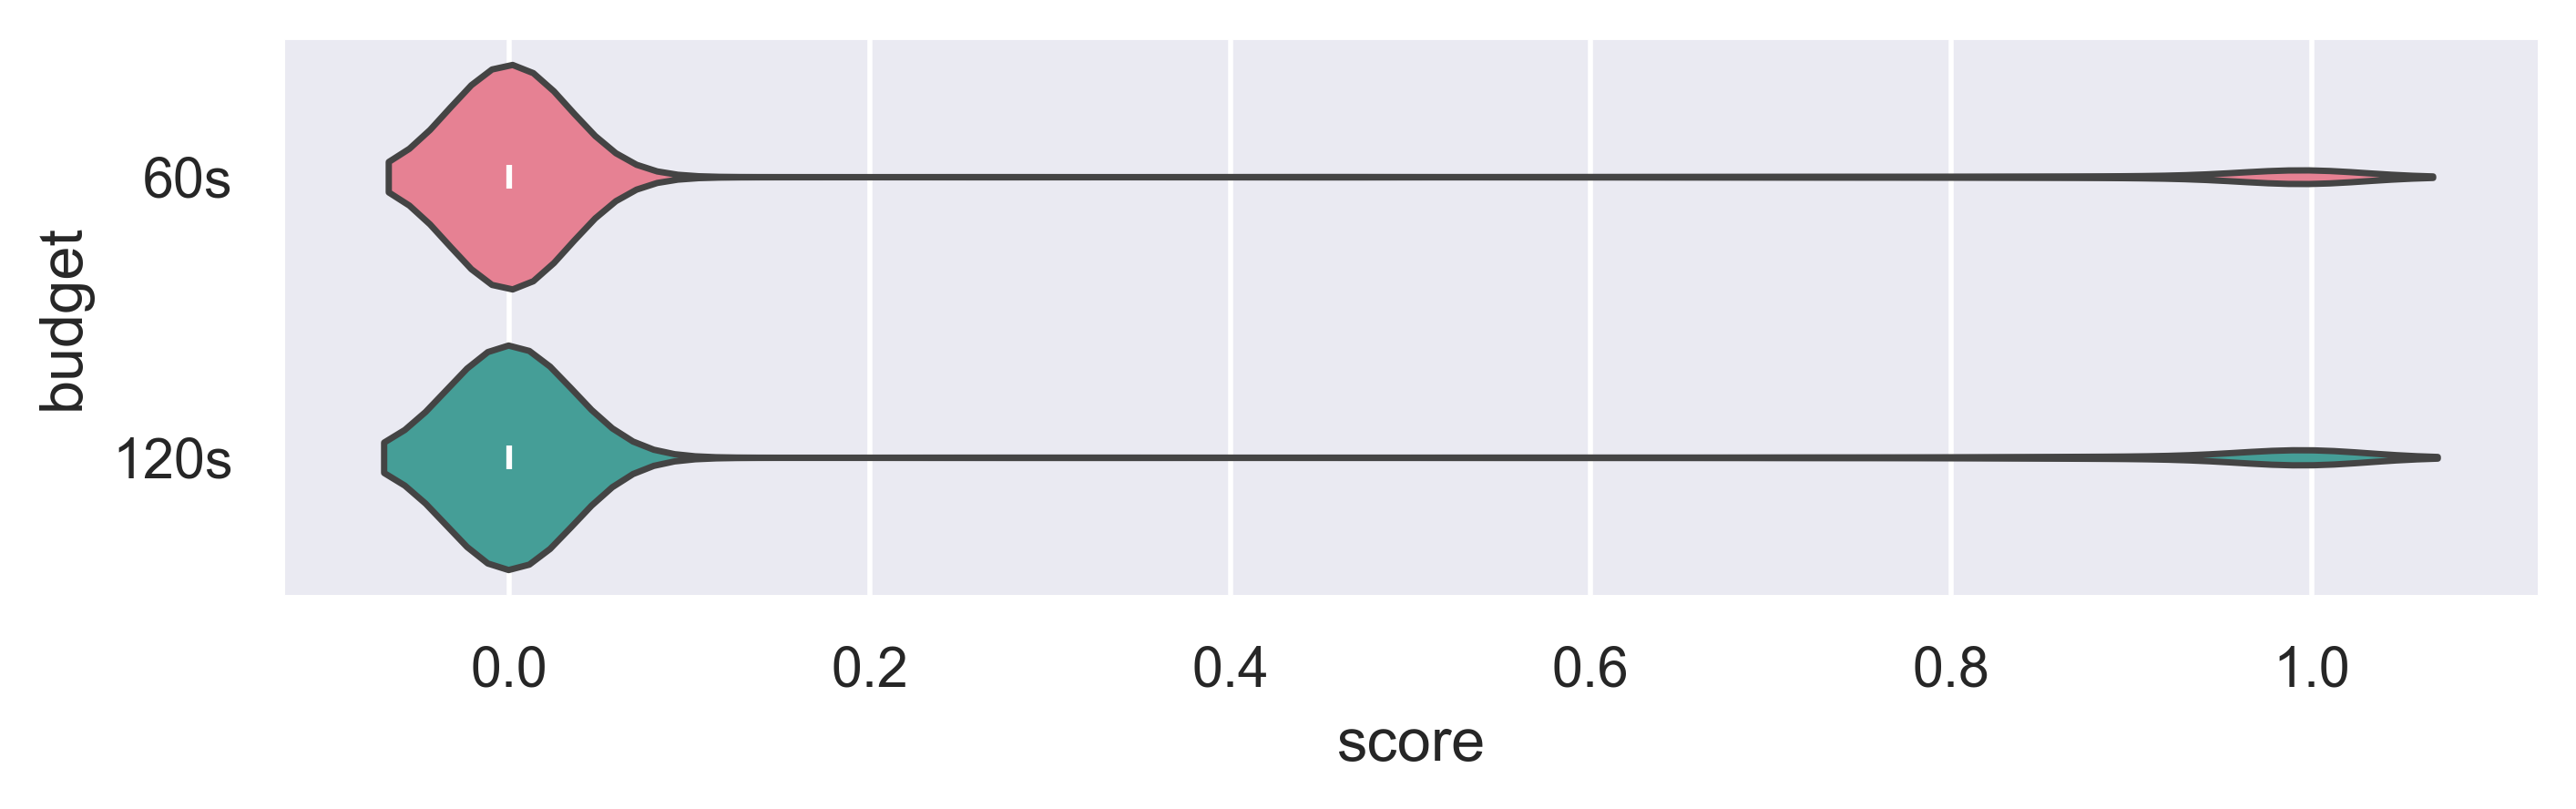
\includegraphics[width=.7\linewidth,keepaspectratio]{../../plots/control_violinplots.png}
\caption{Control violin plots.}
\end{subfigure}

\medskip

\begin{subfigure}{\linewidth}
\centering
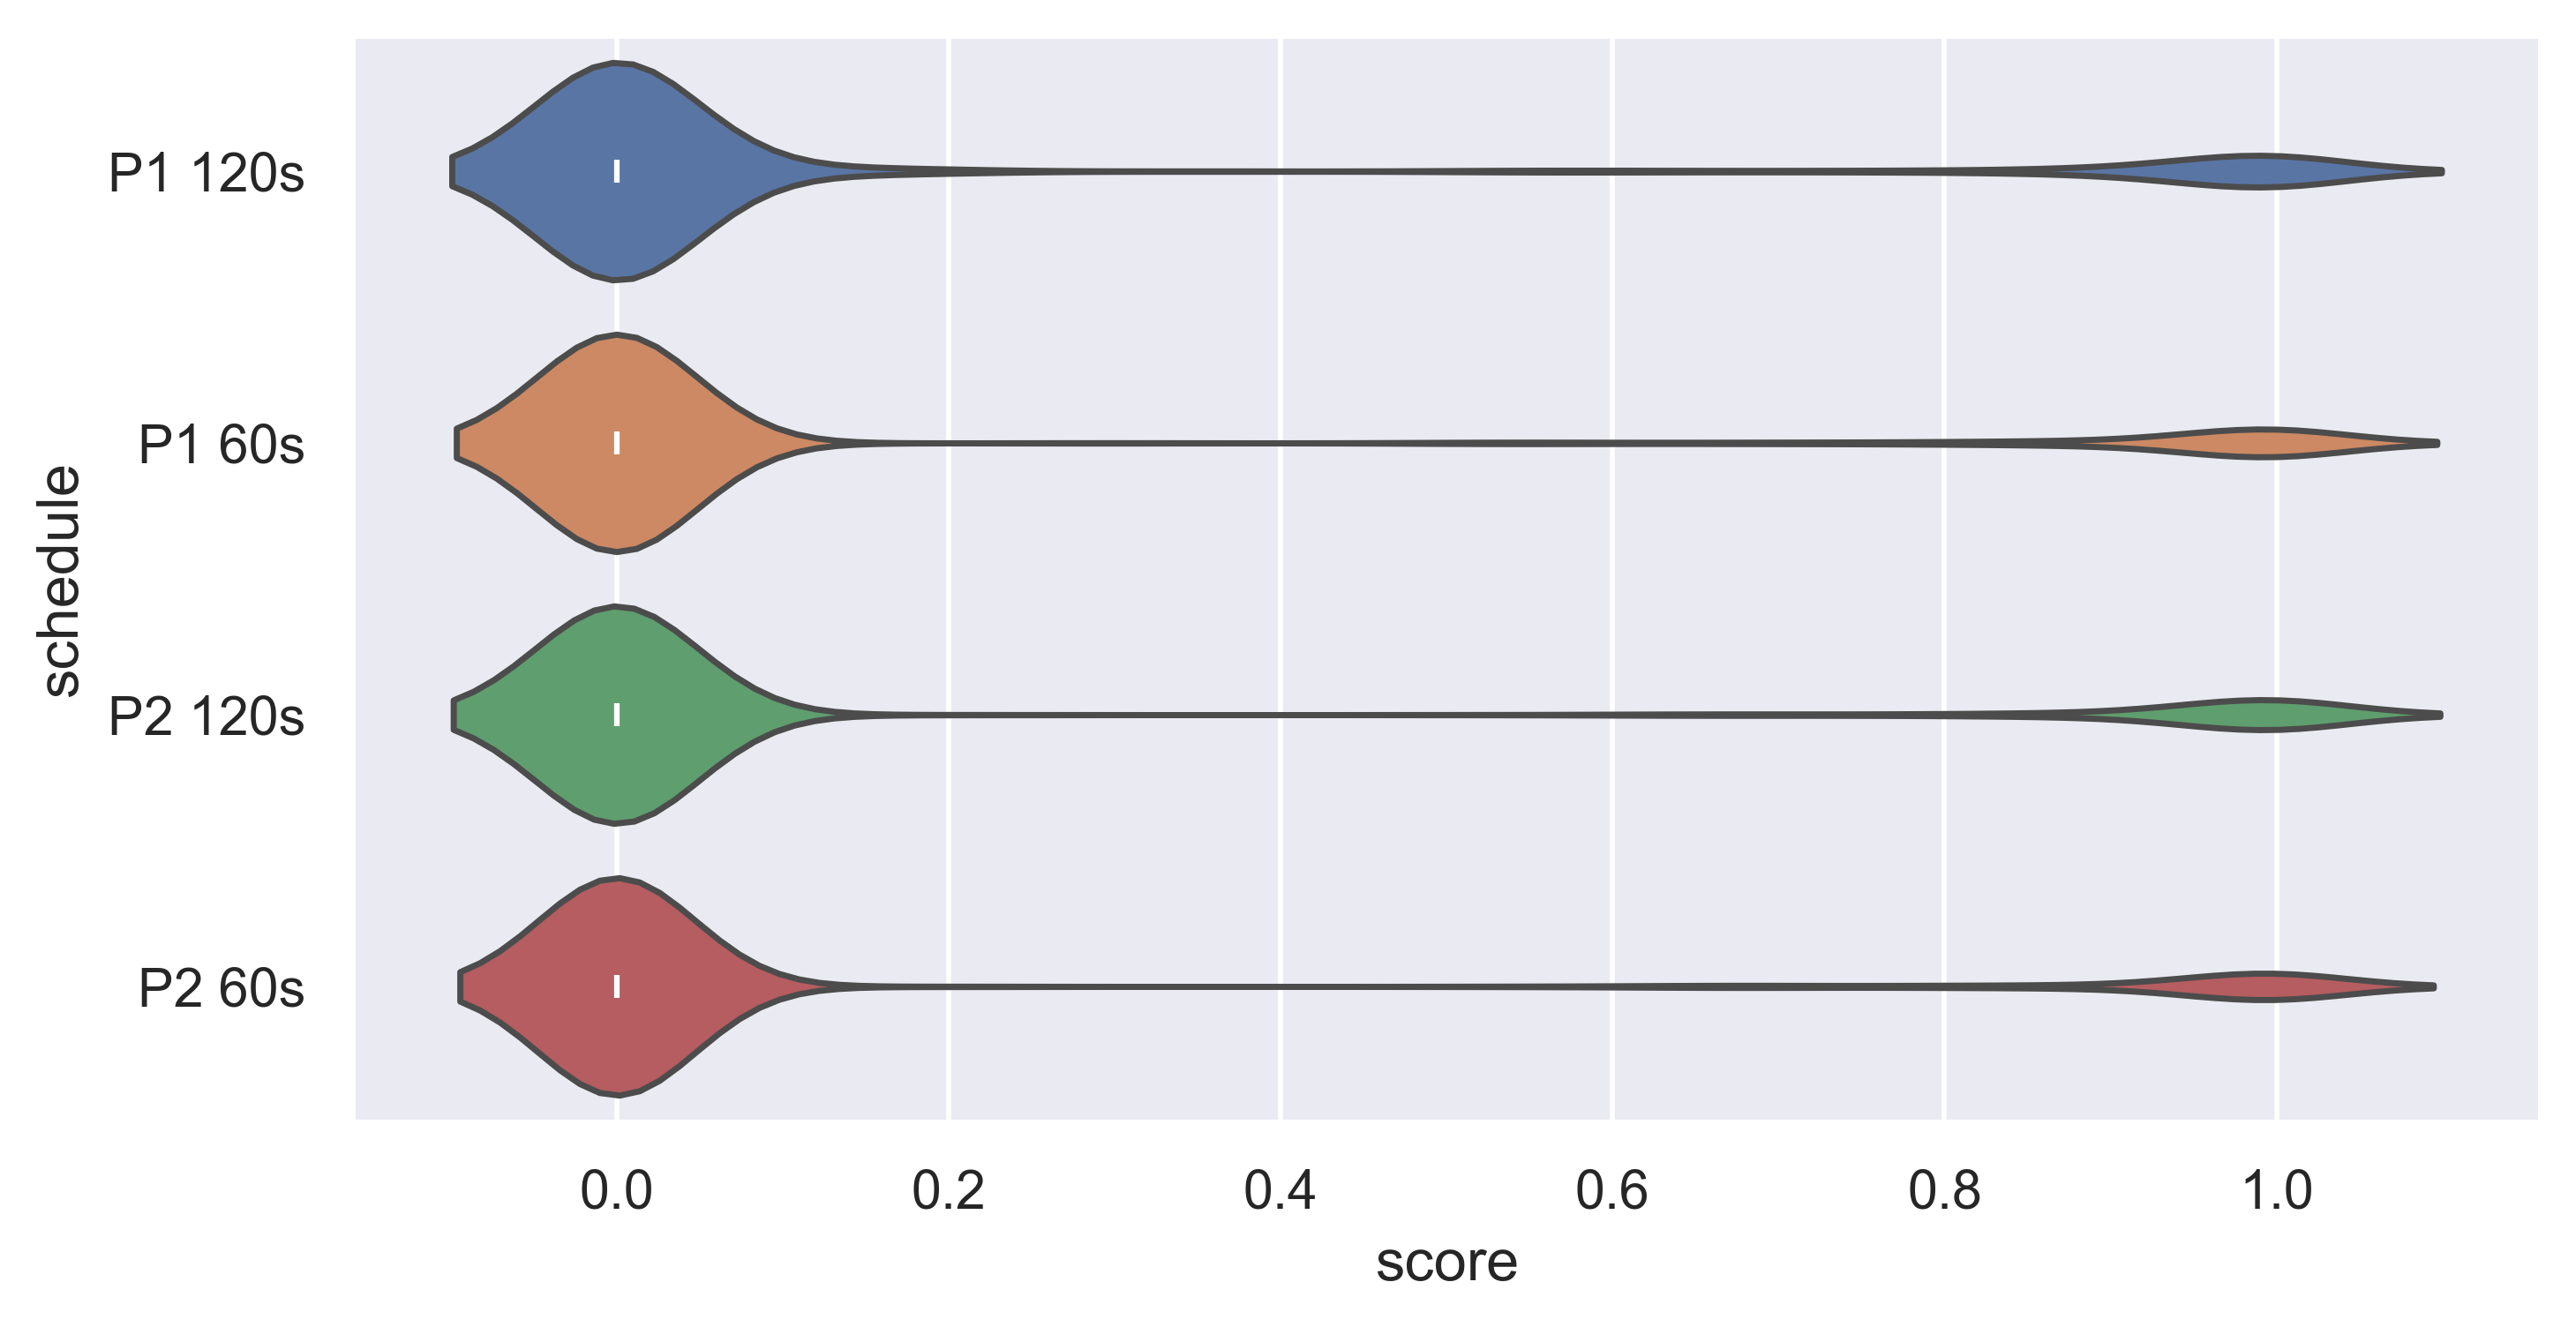
\includegraphics[width=.7\linewidth,keepaspectratio]{../../plots/schedule_violinplots.png}
\caption{Test violin plots.}
\end{subfigure}
\caption{Violin plots of the score distributions. The shorter subfigure shows the controls; the longer subfigure shows the test schedules.}
\label{fig:violins}
\end{figure*}

Each row in \cref{tab:schedule-results} is evaluated at its own global budget.
A portfolio is emulated slot by slot from the measured runtimes: a slot succeeds only if its strategy solves within that slot's cap; otherwise its consumed time is charged and evaluation proceeds.
\emph{Unsolved by \texttt{LeanCopCut}}, \emph{Unsolved by \texttt{FirstAction}}, and \emph{Unsolved by both} are set differences against the budget-matched control solve sets.

\renewcommand*{\bibfont}{\small}
\printbibliography{}

\end{document}
